\documentclass[aspectratio=169]{beamer}
\usepackage{lipsum}
\usepackage[latin,english,brazilian]{babel}
\usetheme{LabIA}

\title{Exemplo de apresentação}
\subtitle{com template LabIA}
\author{Fulano Sicrano da Silva}
\institute{Universidade Federal da Bahia - UFBA}
\date{\today}

\begin{document}

\begin{frame}
    \titlepage
\end{frame}

\begin{frame}
    \frametitle{Outline}
    \label{contents}
    \tableofcontents
\end{frame}

\begin{frame}
    \frametitle{Acronyms}
    \label{acronyms}
    \begin{description}
        \item[API] Application Programming Interface
        \item[LAN] Local Area Network
        \item[ASCII] American Standard Code for Information Interchange
    \end{description}
\end{frame}

\section{Section 1}
\subsection{Subsection a}
\framesection{Seção 1}{Subseção a}

\begin{frame}
    \frametitle{Title}
    \framesubtitle{Subtitle}
    \lipsum[1][1-9]
\end{frame}

\begin{frame}
    \frametitle{List}
    \begin{itemize}
        \item Point A
        \item Point B
        \begin{itemize}
            \item part 1
            \item part 2
            \begin{itemize}
                \item subpart 1
                \item subpart 2
            \end{itemize}
        \end{itemize}
        \item Point C
        \item Point D \footnote{\lipsum[1][1]}
    \end{itemize}
\end{frame}

\subsubsection{Subsubsection aa}
\begin{frame}
    \begin{enumerate}
        \item Point A
        \item Point B
        \begin{enumerate}
            \item part 1
            \item part 2
        \end{enumerate}
        \item Point C
        \item Point D
    \end{enumerate}
\end{frame}

\subsection{Subsection b}
\framesection{}{Subseção b}

\begin{frame}
    \frametitle{Using Columns}
    \label{usingcols}
    \begin{columns}
        \column{0.4\textwidth}
        \lipsum[2][1-5] \cite{BOSCHINI2022}
        \column{0.4\textwidth}
        \lipsum[3][1-6] \cite{smith2021}
    \end{columns}
\end{frame}

\begin{frame}
    \frametitle{Pictures}
    \begin{figure}
        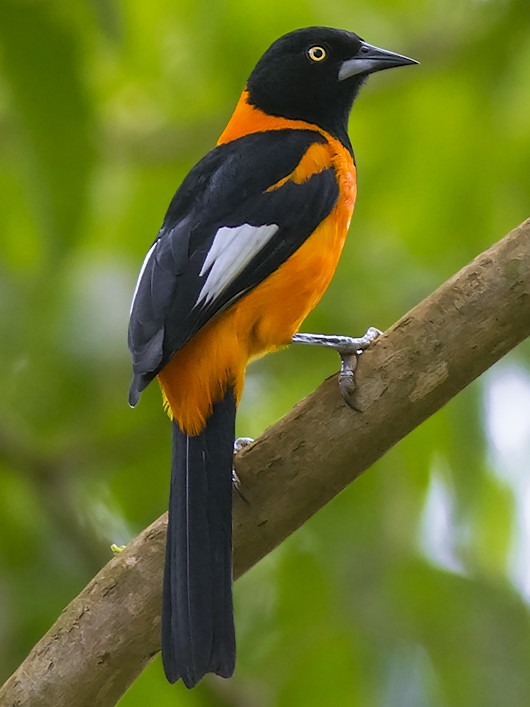
\includegraphics[height=4cm]{sofrê.jpg}
        \caption{\textit{Icterus jamacaii} \cite{wikiaves_corrupiao}}
        \label{image}
    \end{figure}
    \lipsum[4][2-6]
\end{frame}

\begin{frame}
    \frametitle{Table example}
    \begin{table}
        \begin{tabular}{l | c | c | c | c }
            Competitor Name & Swim & Cycle & Run & Total \\
            \hline \hline
            John T & 13:04 & 24:15 & 18:34 & 55:53 \\ 
            Norman P & 8:00 & 22:45 & 23:02 & 53:47\\
            Alex K & 14:00 & 28:00 & n/a & n/a\\
            Sarah H & 9:22 & 21:10 & 24:03 & 54:35 
        \end{tabular}
        \caption{Triathlon results}
        \label{table}
    \end{table}
\end{frame}

\begin{frame}
    \frametitle{Blocks example}
    \begin{block}{Block Title}
        \lipsum[6][1-4]
    \end{block}
    \begin{alertblock}{Block Title}
        \lipsum[6][5-8]
    \end{alertblock}
\end{frame}

\begin{frame}
    \frametitle{Blocks example (cont.)}
    \begin{definition}
        \lipsum[7][1-4]
    \end{definition}
    \begin{example}
        \lipsum[7][5-8]
    \end{example}
\end{frame}

\section{Section 2}

\framesection

\begin{frame}
    \frametitle{Mathematics}
    \begin{theorem}[Pythagoras] 
        $ a^2 + b^2 = c^2$
    \end{theorem}
    \begin{corollary}
        $ x + y = y + x  $
    \end{corollary}
    \pause
    \begin{proof}
        $\omega +\phi = \epsilon $
    \end{proof}
\end{frame}

\begin{frame}[fragile]
    \frametitle{Including Code}
    \begin{semiverbatim}
\\begin\{frame\}
    \\frametitle\{Outline\}
    \\tableofcontents
\\end\{frame\}
    \end{semiverbatim}
\end{frame}

\begin{frame}
    \frametitle{Buttons}

    \href{https://youtu.be/dQw4w9WgXcQ}{External link (please don't click!)}\\
    \hyperlink{usingcols}{Using columns}\\
    \hyperlink{contents}{\beamerbutton{contents page}}\\
    \hyperlink{acronyms}{\beamergotobutton{acronyms page}}\\
    \hyperlink{image}{\beamerskipbutton{image page}}\\
    \hyperlink{table}{\beamerreturnbutton{table page}}
\end{frame}

\section{Bibliography}
\framesection

\begin{frame}{Bibliography}
    \bibliographystyle{plain}
    \bibliography{ref}
\end{frame}

\end{document}
